\documentclass[11pt,titlepage]{article}
\usepackage[utf8]{inputenc}
\usepackage[dutch]{babel}
\usepackage{amsmath}
\usepackage{amsfonts}
\usepackage{amssymb}
\usepackage{graphicx}
\usepackage[table,xcdraw]{xcolor}
\usepackage[toc,page]{appendix}
\usepackage{hyperref}
\usepackage{listings}
\usepackage{float}
\usepackage{tikz}
\usetikzlibrary{trees}
\usepackage{tikz-qtree}
\usepackage{graphicx}
\usepackage{fancyref}
\usepackage{wrapfig}
\usepackage{url}
\usepackage{pdflscape}
\usepackage{fancyvrb}
\graphicspath{ {Afbeeldingen/} }
\usepackage{subfig}
\usepackage{tabularx}
\usepackage{parskip}

\newcolumntype{L}[1]{>{\raggedright\arraybackslash}p{#1}}

%% Sets page size and margins 
\usepackage[a4paper,top=3cm,bottom=3cm,left=3cm,right=3cm,marginparwidth=1.75cm]{geometry}

\author{René van Eendenburg 561378 \cr Derk Wiegerinck 567665}

\title{Ontwerp Documentatie}
\usepackage{titling}

\newcommand{\subtitle}[3]{%
	\posttitle{%
		\par\end{center}
	\begin{center}\large#1\end{center}
	\begin{center}\large#2\end{center}
	\begin{center}\large#3\end{center}
	\vskip0.5em}%
}

\subtitle{HAN Arnhem}{Versie 1}{WOR-World}

\frenchspacing
\sloppy
\begin{document}
\maketitle



\tableofcontents
\clearpage


\section{Inleiding}
In dit document wordt het ontwerp van de uitwerking van de simulatieopdracht beschreven. Hier zal worden ingegaan op de structuur van de packages, Dit houdt in dat alle nodes, topics en messages worden beschreven. Ook wordt beschreven wat de samenhang is van de broncode. Dit wordt met behulp van class diagrams en beschrijvingen van de classes gedaan. Daarnaast wordt er beschreven hoe het gedrag van de belangrijke componenten gerealiseerd is. Tot slot wordt de API van alle publieke interfaces beschreven.

\section{Beschrijving van de packages}
De uitwerking bestaat uit twee ROS-packages: al5d\_simulation en cup. In de volgende paragrafen worden de packages beschreven.

\subsection{al5d\_simulation}
De al5d\_simulation package bevat een node die de al5d controller simuleert en de visualisatie van de lynxmotion al5d.

De controller accepteert berichten van het \href{https://www.robotshop.com/media/files/pdf2/lynxmotion_ssc-32u_usb_user_guide.pdf
}{SSC32U}-format op een rostopic. Het rostopic, genaamd ``SSC32U\_request\_topic'', handelt alle mogelijke requests af. Responses zijn op dit moment niet geïmplementeerd, omdat dit buiten de scope van de opdracht ligt.

Bij een request zal de al5d\_simulation de SSC32U requests converteren en vervolgens publiceren op het ``joint\_state\_message\_topic''. Deze worden op hun beurt weer afgehandeld door de ``robot\_state\_publisher''. Dit topic zal de robot in de Rviz-visualisatie aansturen.

\subsection{cup}
De cup package bevat een node die een beker kan simuleren. De cup luistert naar de frames die de al5d\_simulation publiceert. In de volgende sectie wordt uitgelegd wat de relevante frames zijn en waarom.

\subsubsection{Relevante frames}
De cup maakt gebruik van de door al5d\_simulation gepubliceerde transform-frames van de robot. De belangrijke frames waar de cup geïnteresseerd in is, zijn: ``odom'', ``gripper\_right'' en ``gripper\_left''.

``odom'' is het frame van de simulatie dat altijd vast staat. Met behulp van dit frame, worden de posities van de beker in de gesimuleerde wereld berekend.

De andere twee frames zijn de gripper-frames die worden gebruikt om de positie van de beker ten opzichte van de gripper te bepalen. Ook worden deze frames gebruikt om sensoren aan de gripper te koppelen (dit wordt verderop in het document uitgelegd).

\subsubsection{Verschillende onderdelen van de cup}

De beker bestaat uit een marker en een transform-frame. De marker is een visuele representatie van de beker. Dit bepaalt hoe de beker eruitziet. Aan de hand van het transform-frame wordt bepaalt waar de beker precies is in de gesimuleerde wereld.

Om te bepalen wanneer de beker opgepakt is, zijn er ``sensoren'' gerealiseerd op de gripper. Dit zijn markers die de positie van de grippers met een bepaalde offset volgen. Als de sensoren de beker detecteren, is de cup opgepakt. Ook zijn er twee sensoren gerealiseerd aan de buitenkant van de grippers. Op deze manier kan de beker verschoven worden. Deze sensoren bepalen uiteindelijk de toestand van de beker. De volgende toestanden zijn mogelijk: opgepakt, niet opgepakt, schuiven naar links en schuiven naar rechts.

Na het bepalen van de toestand, kunnen er een aantal zaken worden gedaan. Als de beker niet opgepakt is, wordt er een zwaartekracht gesimuleerd. Dit zorgt ervoor dat als de positie van de beker boven de grond is, de positie wordt verminderd met een factor totdat de beker de grond heeft bereikt. Als de beker opgepakt is, wordt het transform-frame van de beker gekoppeld aan de gripper, zodat de beker de gripper volgt. Dit wordt ook gedaan in de overige toestanden.

Elke cup publiceert zijn snelheid, versnelling en oriëntatie op topics in de vorm van ``cup'' + id + ``\_'' + (``speed'' / ``velocity'' of ``orientation''). Daarnaast wordt de marker van de cup wordt gepubliceerd zodat deze zichtbaar is in de wereld en het transform-frame wordt gepubliceerd. De cup publiceert ook de sensors (deze bestaan ook uit visuele markers en transform-frames). De markers zijn in de simulatie te zien als ``left\_sensor'', ``right\_sensor'', ``left\_outer\_sensor'' en ``right\_outer\_sensor''. 

\subsubsection{Starten van de cup}
Om een beker in de simulatie wereld te weergeven, moeten de volgende argumenten worden meegegeven. Een numeriek ID, X locatie, Y locatie en een Z locatie. 

\section{Structuur van de packages}

\subsection{al5d\_simulation}

De al5d is opgezet in de volgende onderdelen. Een command parser, servo aansturing, een publisher en een controller klasse. Na het klassediagram zal er een kleine beschrijving van elk onderdeel staan.

\begin{figure}[H]
\centering
    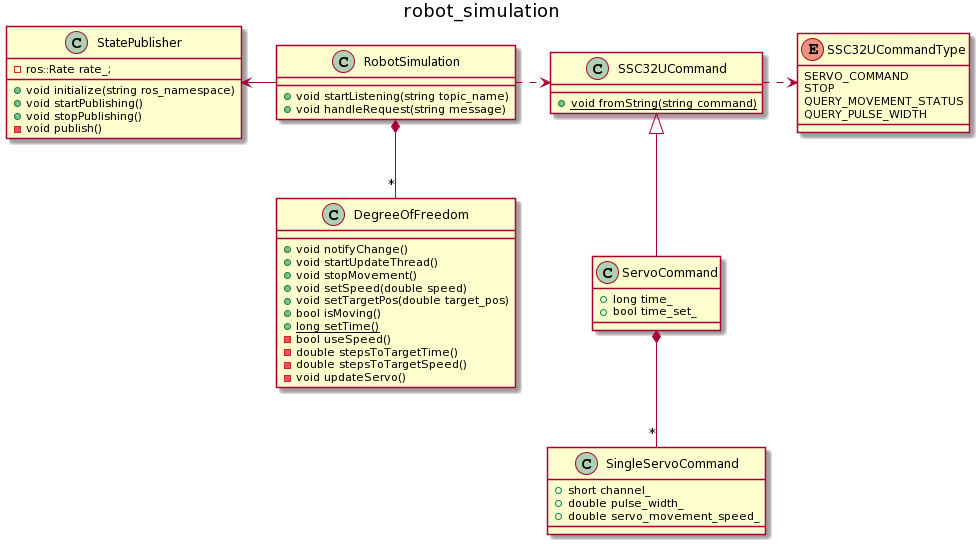
\includegraphics[scale = .4]{robot_sim_plantuml.png}
    \caption{al5d\_simulation class diagram}
    \label{figure:al5d_simulation}
\end{figure}

\subsubsection{SSC32UCommand}
Deze klasse parsed SSC32U string commando's en geeft een SSC32U object terug. Dit object kan een ServoCommand zijn, deze kan meerdere SingleServoCommands bevatten. Hierin zitten het kanaal voor de servo, de gewenste positie en de snelheid voor de servo. In een ServoCommand kan ook een globale tijd worden gezet. De keus voor individuele servo snelheid of de globale tijd wordt gebruikt, wordt afgehandeld in DegreeOfFreedom.

\subsubsection{DegreeOfFreedom}
Een object van deze klasse dient als een enkele servo. De servo ontvangt een target positie waar de servo naar toe moet bewegen. De servo zal vervolgens berekenen, op basis van de gegeven snelheid, tijd of limitaties van de servo, in hoe veel stappen er bewogen wordt naar de target positie. De limitaties van de servo worden opgehaald van de Ros Parameter server. Deze parameter server wordt geladen met een xarco file.

\subsubsection{StatePublisher}
Deze klasse benodigd een lijst met alle servo's. Vervolgens zal deze met een vaste rate door de lijst heen loopen in de functie Publish en daarmee de configuratie van de robot arm doorsturen naar het "joint\_state\_message\_topic".

\subsubsection{RobotSimulation}
De RobotSimulation is de controller van de al5d\_simulation. Deze handelt de requests af die binnen komen op het rostopic.

\subsection{cup}

De cup bestaat uit een aantal onderdelen: de classes voor de marker, classes voor de sensor en de overige classes. In de code zijn deze classes onder namespaces verdeeld. De lege classes zijn verwijzingen naar classes die behoren tot een andere namespace.

\begin{figure}[H]
\centering
    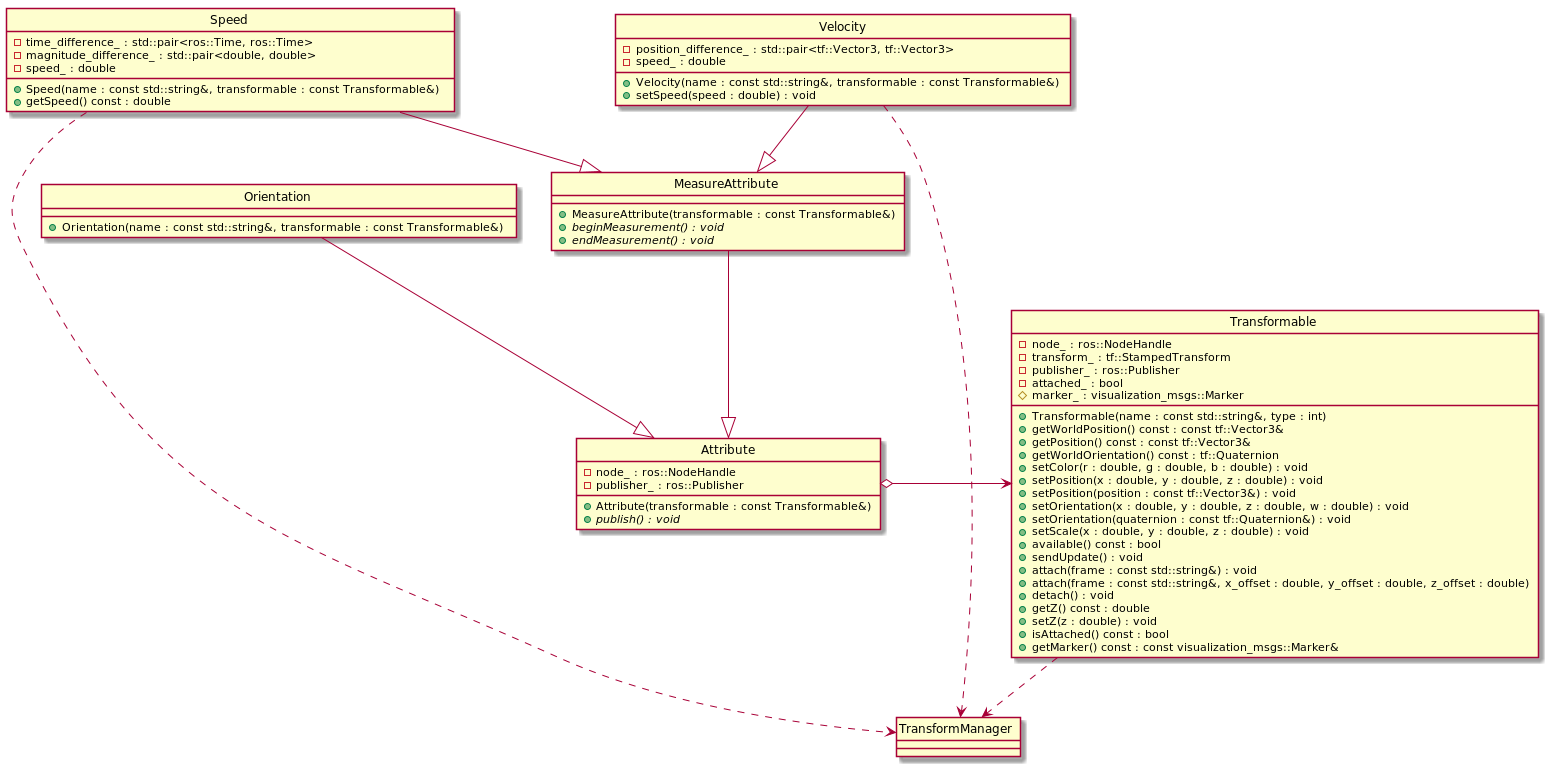
\includegraphics[scale = .25]{cup_class_diagram_marker.png}
    \caption{cup class diagram van de marker}
    \label{figure:cup_class_diagram_marker}
\end{figure}

In \autoref{figure:cup_class_diagram_marker} zijn de classes weergeven die behoren tot de namespace marker. Dit bevat alle functionaliteit van een marker: de visuele representatie, het transform-frame en attributen van een marker als snelheid, oriëntatie en versnelling.

\begin{figure}[H]
\centering
    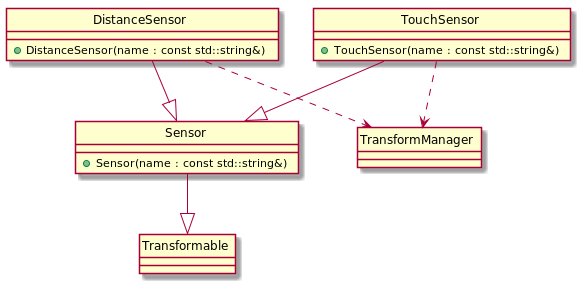
\includegraphics[scale = .5]{cup_class_diagram_sensor.png}
    \caption{cup class diagram van de sensor}
    \label{figure:cup_class_diagram_sensor}
\end{figure}

In \autoref{figure:cup_class_diagram_sensor} zijn de classes weergeven die behoren tot de namespace sensor. Dit bevat alle functionaliteit van een sensor. Een sensor is een marker met een vaste grootte en vorm en kan worden gebruikt om een andere marker (zoals een beker) te detecteren.

\begin{figure}[H]
\centering
    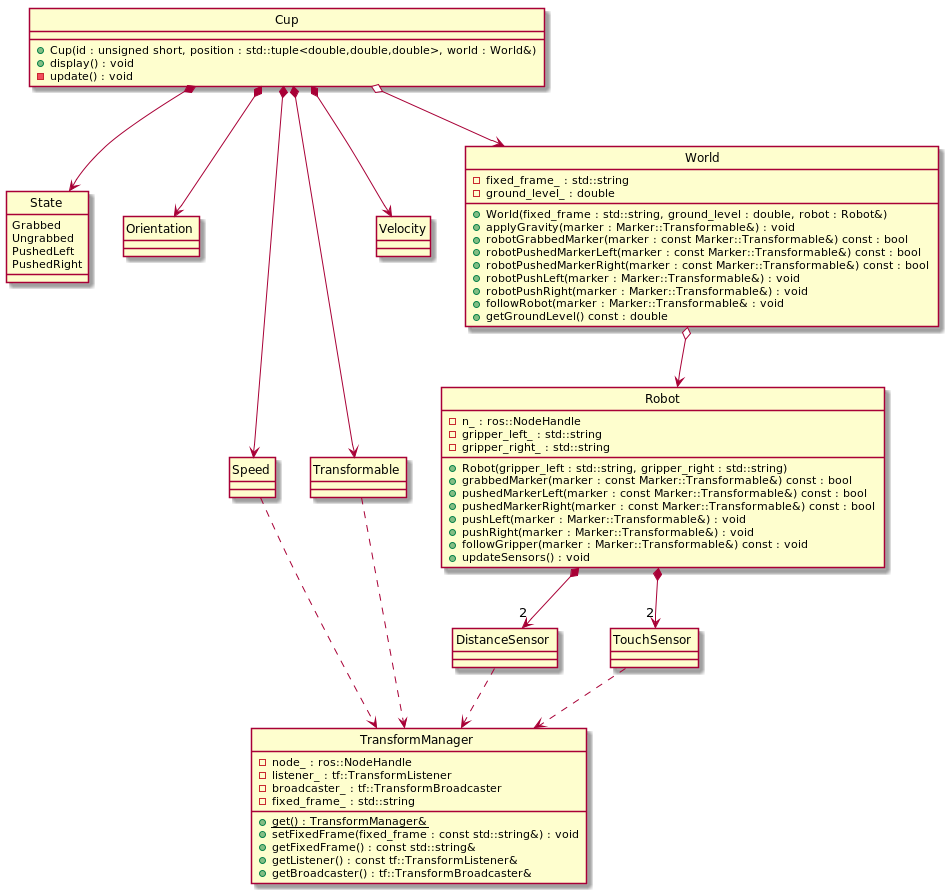
\includegraphics[scale = .3]{cup_class_diagram.png}
    \caption{cup class diagram van de overige classes van de cup}
    \label{figure:cup_class_diagram}
\end{figure}

In \autoref{figure:cup_class_diagram} zijn de overige classes weergeven. Deze zijn niet onderverdeeld in een specifieke namespace. Dit bevat de classes die voornamelijk gebruik maken van de classes van andere namespaces en op zichzelf niet veel functionaliteit toevoegen.

In de volgende secties worden de individuele classes beschreven.

\subsubsection{Attribute}
Deze class definieert een interface om een attribuut van een marker te kunnen maken. Een attribuut is een onderdeel van een marker dat gepubliceerd kan worden. Het bevat het absolute minimum wat benodigd is voor het publiceren van een attribuut.

\subsubsection{MeasureAttribute}
Deze class definieert een interface om een attribuut van een marker te kunen maken, waarbij iets (zoals tijd) gemeten moet worden.

\subsubsection{Transformable}
Deze class bevat een visuele representatie van de marker en het transform-frame van de marker. Het houdt beide representaties bij elkaar. Dit biedt het voordeel als het transform-frame wordt geüpdatet, de visuele represenatie ook wordt geüpdatet.

\subsubsection{Speed}
Deze class kan worden gebruikt om de snelheid te meten van een marker en om dit te publiceren.

\subsubsection{Orientation}
Deze class kan worden gebruikt om de oriëntatie van de marker te meten en te publiceren.

\subsubsection{Velocity}
Deze class kan worden gebruikt om de versnelling van een marker te meten en te publiceren.

\subsubsection{Sensor}
Deze class definieert een interface om specifiekere sensoren te kunnen maken. Het bevat het absolute minimum om een sensor te definiëren. De sensor is een marker van vaste grootte en vorm.

\subsubsection{TouchSensor}
Deze class kan worden gebruikt om te detecteren of een marker de TouchSensor aanraakt.

\subsubsection{DistanceSensor}
Deze class kan worden gebruikt om te detecteren of een marker het midden van de DistanceSensor aanraakt. Het verschil tussen de TouchSensor en DistanceSensor is dat de TouchSensor een collision detecteert als een marker de sensor aanraakt. De DistanceSensor detecteert een collision op basis van het midden van de sensor.

\subsubsection{Cup}
De Cup bevat een marker, verschillende marker-attributen en de toestand van de beker (opgepakt, niet opgepakt, verschoven naar links of rechts). Ook heeft het een referentie naar de World om zo te controleren of de Robot iets met de beker heeft gedaan en om zwaartekracht op de beker toe te kunnen passen.

\subsubsection{World}
De World is een toegangsluik van de Cup naar de Robot. De beker weet in principe niets van de robot, maar weet wel van de wereld. De World heeft een vast transform-frame en weet ook waar de grond is. Daarnaast kan de World zwaartekracht op de Cup toepassen.

\subsubsection{Robot}
De Robot is een representatie van de Robot in het perspectief van de Cup. Het bevat dus ook alleen de voor de Cup relevante transform-frames. Om te kunnen detecteren of de beker is opgepakt of is verschoven, heeft de robot twee DistanceSensors aan de binnenkant van de gripper en twee TouchSensors aan de buitenkant van de gripper.

\subsubsection{TransformManager}
De TransformManager is een singleton zodat classes makkelijker bij de TransformListener en TransformBroadcaster kunnen komen. Ook weet de TransformManager wat het vaste transform-frame is.

\end{document}